\documentclass{ctexbeamer}
\title{公益数据的现状与未来}
\author{赵丰\\ 616545598@qq.com}
\AfterPreamble{\hypersetup{
  colorlinks=false,
}}
\begin{document}
\begin{frame}
\titlepage
\end{frame}
\begin{frame}
\frametitle{概要}
\tableofcontents
\end{frame}
\section{主题背景}
\begin{frame}% the link may not be permanent
\frametitle{\href{http://www.ixueshu.com/document/332c6697f89ecc79318947a18e7f9386.html}{“WA”,IBM企业社会责任聚焦“公益大数据”}}
\begin{figure}

\includegraphics[width=\textwidth]{background1.jpeg}
\end{figure}
\end{frame}
\begin{frame}
\begin{quote}
参与者针对“志愿者管理”、“筹款募捐”、“社区参与”场景下的提升目标,用WA对样本数据进行分析,依据分析结果制定改善方案。
\begin{flushright}
《社会与公益》2016年7月刊
\end{flushright}
\end{quote}
\begin{quote}
合作伙伴“灵析”是目前国内快速崛起、影响力最大的公益机构数据服务提供商,其捐赠人、志愿者Saas产品服务超过3000家机构。
\begin{flushright}
\href{http://www.sohu.com/a/106631644_350071}{搜狐新闻,公益中国2016年7月19号}
\end{flushright}
\end{quote}
\end{frame}
\begin{frame}% the link may not be permanent
\frametitle{\href{http://www.sohu.com/a/190256051_247771}{“中国公益基金会数据骇客马拉松竞赛”圆满落幕 }}
\begin{figure}
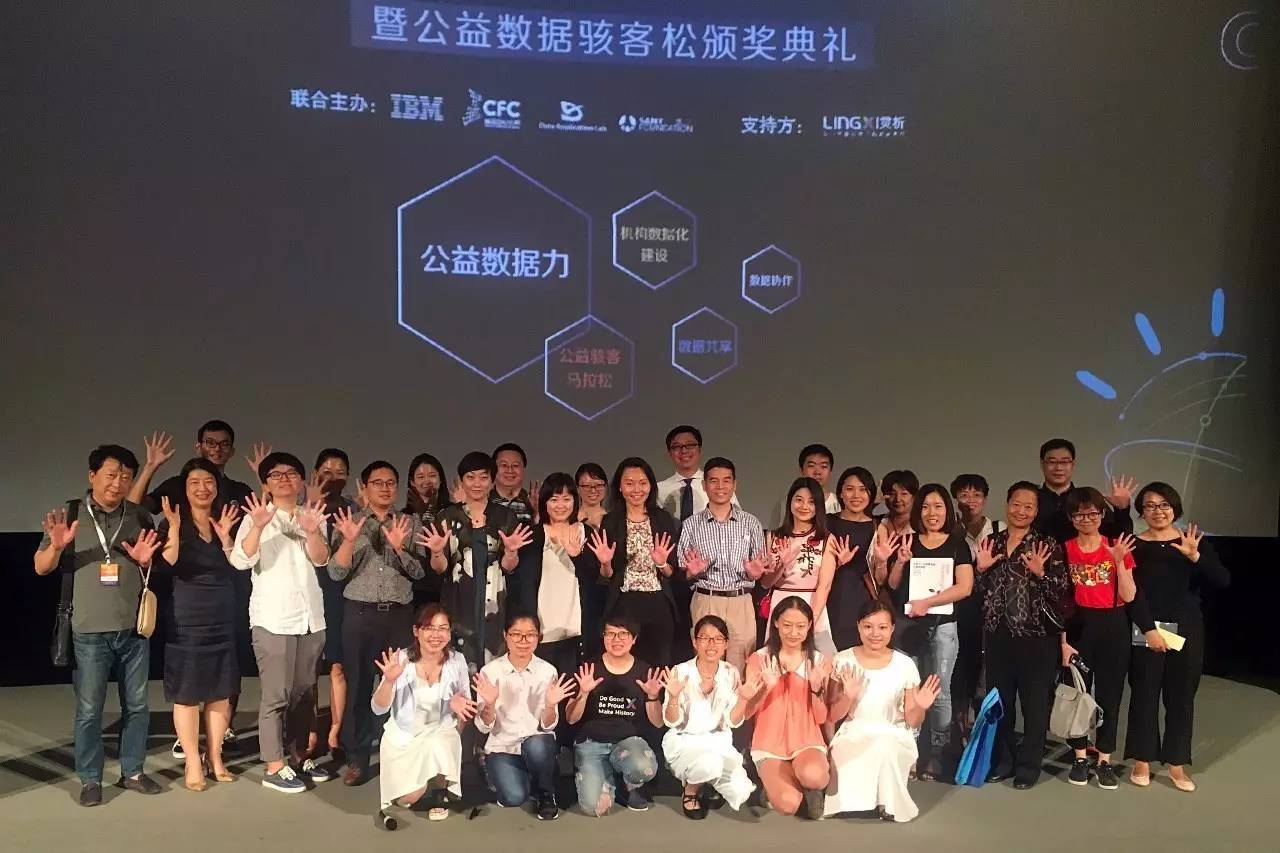
\includegraphics[width=\textwidth]{background2.jpeg}
\end{figure}
\end{frame}
\begin{frame}
\begin{quote}
当下社会对数据科学的热情主要集中在金融,互联网,医疗等热点,却忽视了公益领域的需求,这种局面需要得到改变。
\begin{flushright}
搜狐新闻,基金会中心网2017年9月6日\\
引用DAL数据应用学院联合创始人陈晓理
\end{flushright}
\end{quote}
\begin{center}
\href{http://www.foundationcenter.org.cn/data_hackthrone/index.html}{竞赛选题}
\end{center}
\begin{enumerate}
\item 基金会中心网推荐系统:从公司与基金会的需求出发
\item 舆情分析:社会大众对基金会的认知及公益基金会社会影响力
\end{enumerate}
\end{frame}
\begin{frame}
\frametitle{\href{http://mp.weixin.qq.com/s/2XXehZ4KlFKT7FuEqluY3w}{数说志愿 | 你真的了解清华31支紫荆支队吗? }}
\begin{figure}
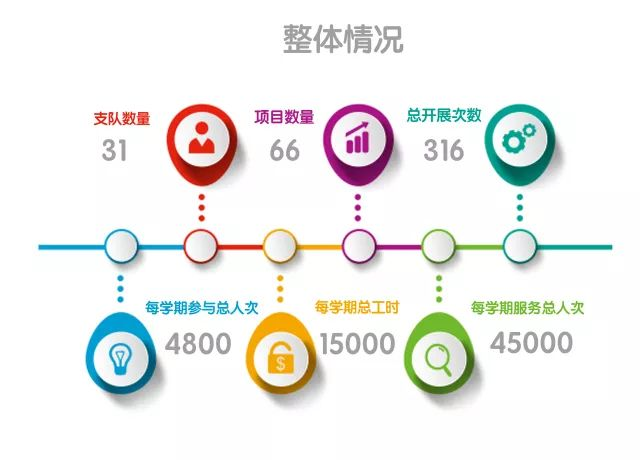
\includegraphics[width=\textwidth]{background3.jpg}
\end{figure}
\end{frame}
\begin{frame}
\begin{quote}
目前,清华共有31支紫荆支队,它们分别属于各自院系团委,开展各种院系志愿活动并承接部分志愿中心活动。目前总共运营了66个项目,每学期开展次数300多次,参与人次4800以上,帮助了超过45000人。
\begin{flushright}
清华大学学生公益官方微信2017年12月24日
\end{flushright}
\end{quote}
日前,笔者统计在志愿北京官网上,清华大学学生公益活跃的支队共有42个,参与总人次为 21625人,运营项目共计1679个。
%mysql> select project.project_id from project, organization where project.organization_id = organization.organization_id and organization.upper_organization_id %%= 3472185;
% 3472185 是 总会的org id.
\end{frame}

\begin{frame}
\frametitle{公益数据的价值}% 动机不足
\begin{itemize}
\item 从公益数据中学习,未来我们可以做得更专业 % example? imagination
% 争议:公益主要靠人,靠组织,组织能力、爱心等不可能从数据中学习,做公益,无记忆性更多一点
\item 利用数据学习技术,辅助志愿组织、志愿者双向匹配,辅助捐赠人、NGO双向匹配。
%\item 各大组织对公益数据的重视程度在增加。
\end{itemize}
\end{frame}


\section{公益数据平台}
\begin{frame}
\frametitle{\href{https://www.lingxi360.com/}{灵析-每个智慧公益背后都有灵析}}
\begin{figure}
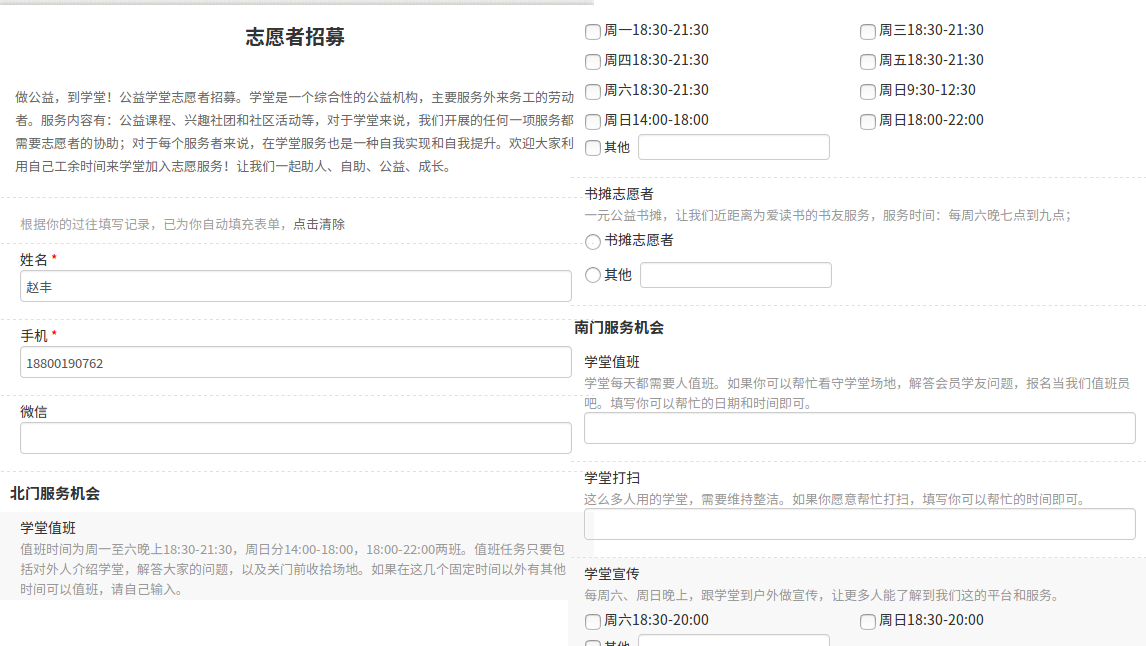
\includegraphics[width=\textwidth]{data1.png}
\caption{深圳清湖社区学堂招募令(灵析表单)}
\end{figure}
\end{frame}
\begin{frame}
\frametitle{\href{http://gongyi.qq.com/jjhgy/about/about.htm}{腾讯公益}}
\begin{figure}
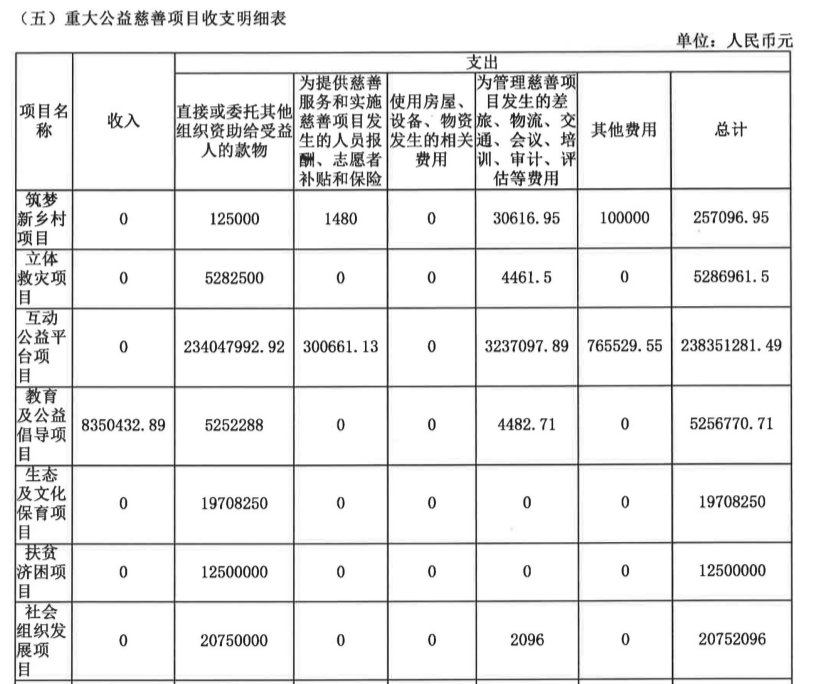
\includegraphics[width=0.8\textwidth]{data2.png}
\caption{腾讯基金会2016年工作报告第25页}
\end{figure}
%支付宝公益类似
\end{frame}
\begin{frame}
\frametitle{\href{http://www.bv2008.cn}{志愿北京}}
\begin{figure}

\includegraphics[width=\textwidth]{data3.png}
\caption{\href{http://www.bv2008.cn/app/opp/view.php?id=147076}{助力西站项目}}
\end{figure}

%志愿深圳类似,但功能弱。
\end{frame}
\begin{frame}
\frametitle{数据来源小节}
\begin{itemize}
\item 腾讯和支付宝平台分割公益捐赠数据
\item 灵析在NGO招募志愿者数据方面独占鳌头
\item 城市服务数据由全国志愿系统牢牢掌控
\item 基金会数据可在\href{http://www.foundationcenter.org.cn/}{基金会中心网}上查到
\end{itemize}
%\begin{center}
%存在的问题
%\end{center}
%\begin{itemize}
%\item 出于隐私保护,涉及志愿者个人信息的数据最多部分公开% 但这一点有可能成为公益数据分析的关键,
%\item 各平台的数据无法统一,而人的活动往往涉及多个平台
%\end{itemize}
\end{frame}
\section{聚焦大学生公益} %大学生=本科生
\begin{frame}
\frametitle{大学生=本科生?}
\begin{figure}
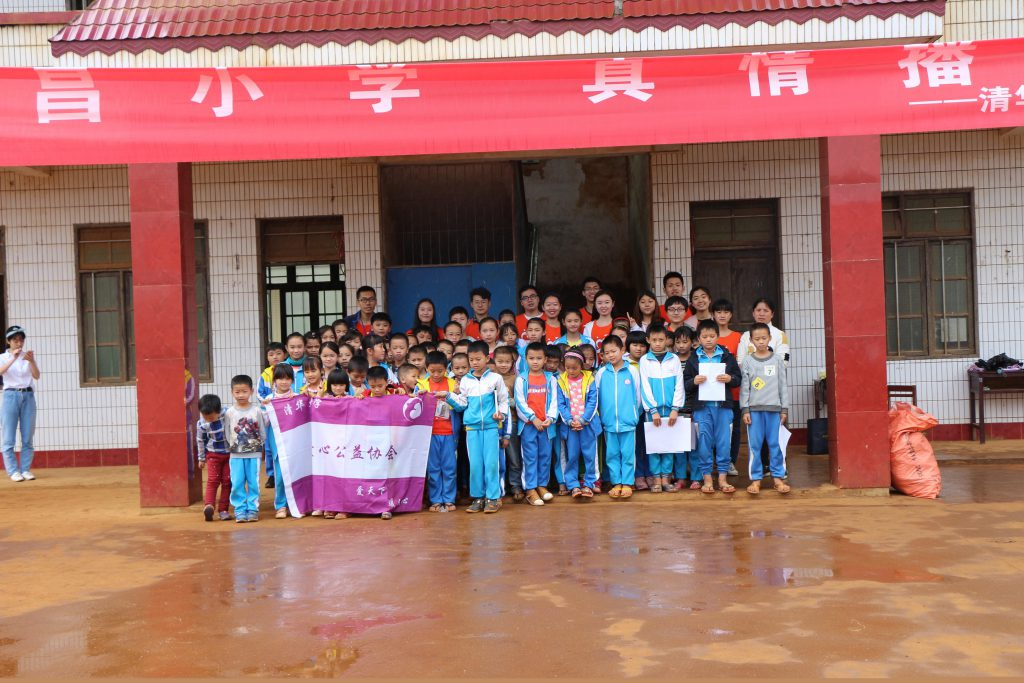
\includegraphics[width=\textwidth]{student1.jpg}
\caption{\href{http://leidenschaft.cn/volunteer0/}{清华爱协2018寒假赴海南文昌新桥大昌小学支教}}
\end{figure}
\end{frame}
\begin{frame}
\frametitle{大学生公益=公益支教?}
\begin{quote}
参加志愿者活动中,在校大学生是支教志愿者主体,占总人数的55.29\%。
\begin{flushright}
\href{http://www.cta613.org/thread-9282-1-1.html}{中华支教与助学信息中心民间支教报告}\\2016年6月13日
\end{flushright}
\end{quote}
\begin{figure}
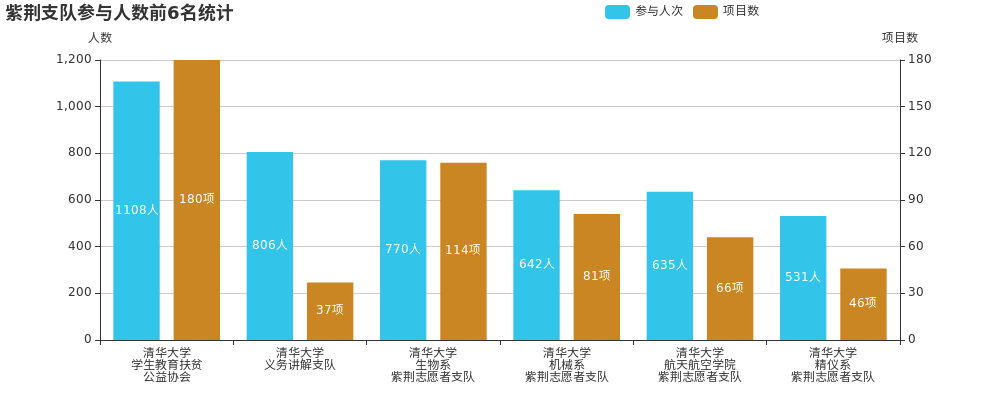
\includegraphics[width=\textwidth]{student2.png}
\end{figure}
\end{frame}
\begin{frame}
\frametitle{大学生公益数据现状}
\framesubtitle{NGO或高校社团有自己的不对外公开的内部数据,但数据无法对比}
\begin{quote}
十年以来,美在心灵安排志愿者1.9万人次,服务小学754所次,受益学生6.2万人次,总服务时长165万小时,总投入善款158万元。
\begin{flushright}
\href{http://mp.weixin.qq.com/s/6gOQS-SN3P4PHH27FCMFTQ}{海南省“美在心灵”大学生支教志愿者协会官方简介}
\end{flushright}
\end{quote}
\begin{figure}
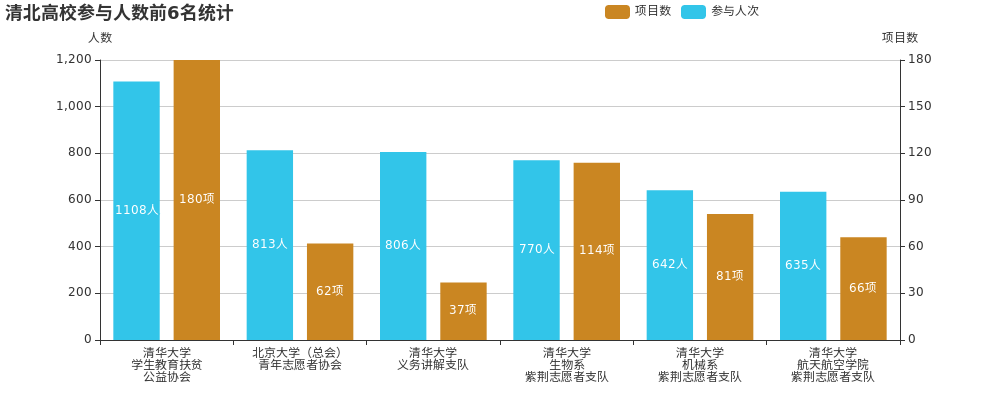
\includegraphics[width=\textwidth]{student3.png}
\end{figure}
\end{frame}
\begin{frame}
\frametitle{男女比例是否可以信赖?}
\begin{quote}
在参与支教活动的人员中,又以女性居多,占总人数的 77.6\%。
\vspace{-0.1cm}
\begin{flushright}
{\small\href{http://www.cta613.org/thread-9282-1-1.html}{中华支教与助学信息中心民间支教报告}2016年6月13日}
\end{flushright}
\end{quote}
\vspace{-0.45cm}
\begin{figure}
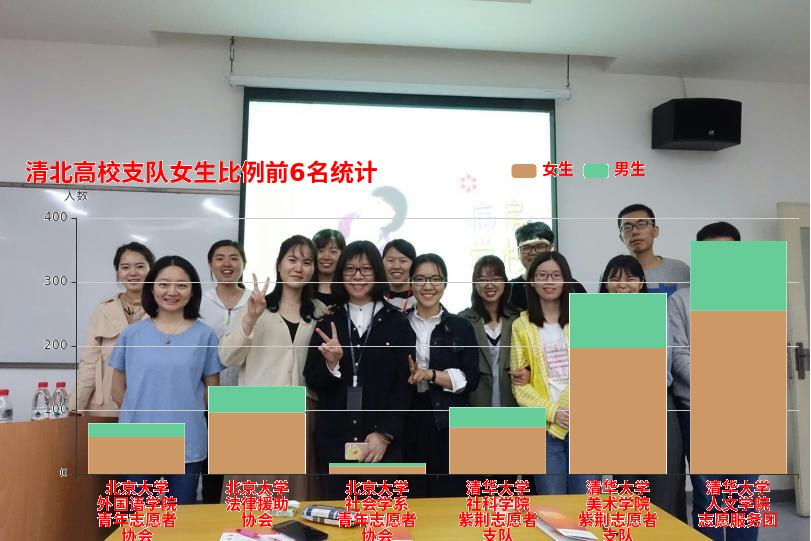
\includegraphics[width=0.8\textwidth]{all.jpg}
\caption{南燕青协:“新阳光病房”第一次志愿者培训}
\end{figure}
\end{frame}
\begin{frame}
\frametitle{\href{http://data-visualization.leidenschaft.cn/bv2008.html}{清北支队}}
\begin{itemize}
\item 与院系人数、男女比例密切相关
\item 历年波动大,与组织者一年一换届有关
\end{itemize}
\begin{figure}
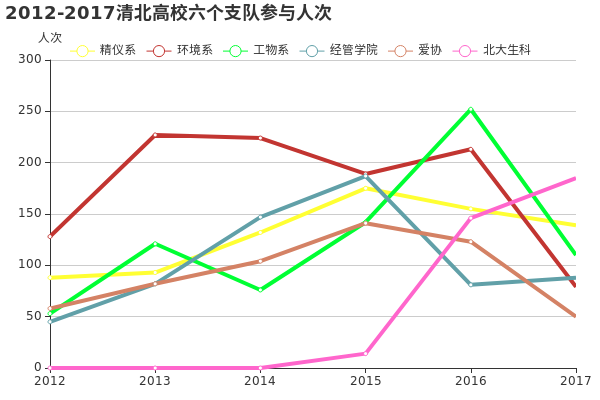
\includegraphics[width=0.8\textwidth]{student5.png}
\end{figure}
\end{frame}
\section{公益数据展望}%personal view
\begin{frame}
\frametitle{公益数据展望}
\begin{itemize}
\item 信赖的数据源.%:如果志愿北京数据也可以造假。
\item 有效的公益数据收集机制。%:清华深研院紫荆志愿者团尚未融入志愿深圳义工系统中。
\item 统一、透明的平台。%:志愿深圳和志愿北京是两套系统,志愿深圳系统的透明度偏低。
\item 从传统的问卷小样本到平台数据分析:路还很漫长。
\end{itemize}
\begin{figure}
\centering

\includegraphics[width=\textwidth]{footer.png}
\end{figure}
\end{frame}
% beamer official guide suggests providing short, important bibliography at the end of the presentation, which can fit one slide
% present references only if they are intended as "further reading"
% no bib given.
\end{document}
